\documentclass[11pt,a4paper]{article}

% ─── Packages ────────────────────────────────────────────────────────────────
\usepackage[T1]{fontenc}
\usepackage[utf8]{inputenc}
\usepackage{lmodern}
\usepackage{microtype}
\usepackage[margin=2.5cm]{geometry}
\usepackage{amsmath,amssymb,amsthm}
\usepackage{bm}
\usepackage{booktabs}
\usepackage{array}
\usepackage{graphicx}
\usepackage{xcolor}
\usepackage{hyperref}
\usepackage[round]{natbib}
\usepackage{enumitem}
\usepackage{listings}
\usepackage{caption}
\usepackage{subcaption}
\usepackage{tikz}

% ─── Hyperref setup ──────────────────────────────────────────────────────────
\hypersetup{
  colorlinks  = true,
  linkcolor   = blue!60!black,
  citecolor   = teal!70!black,
  urlcolor    = blue!70!black,
  pdftitle    = {Basanos: Correlation-Aware Signal Assessment for Systematic Strategies},
  pdfauthor   = {Jebel Quant},
}

% ─── Code listing style ──────────────────────────────────────────────────────
\lstset{
  basicstyle   = \ttfamily\small,
  keywordstyle = \bfseries\color{blue!70!black},
  commentstyle = \itshape\color{gray!70},
  stringstyle  = \color{teal!70!black},
  breaklines   = true,
  frame        = single,
  framerule    = 0.4pt,
  xleftmargin  = 1em,
  xrightmargin = 1em,
}

% ─── Math macros ─────────────────────────────────────────────────────────────
\newcommand{\C}{\mathbf{C}}
\newcommand{\I}{\mathbf{I}}
\newcommand{\x}{\mathbf{x}}
\newcommand{\muvec}{\bm{\mu}}
\newcommand{\R}{\mathbb{R}}
\newcommand{\norm}[1]{\left\|#1\right\|}
\newcommand{\abs}[1]{\left|#1\right|}
\DeclareMathOperator{\tr}{tr}
\DeclareMathOperator{\rank}{rank}
\DeclareMathOperator{\eff}{eff\text{-}rank}
\newcommand{\Bload}{\mathbf{B}}
\newcommand{\Ffac}{\mathbf{F}}
\newcommand{\Dspe}{\mathbf{D}}

\newtheorem{remark}{Remark}
\newtheorem{proposition}{Proposition}

% ─── Title ───────────────────────────────────────────────────────────────────
\title{%
  \textbf{Basanos: Correlation-Aware Signal Assessment\\
  for Systematic Strategies}\\[0.5em]
  \large A Companion Paper
}
\author{Jebel Quant}
\date{\today}

% ─────────────────────────────────────────────────────────────────────────────
\begin{document}

\maketitle

\begin{abstract}
Raw trading signals produced by forecasting models encode directional views
about asset returns, but they carry no information about portfolio correlation
structure.  Sizing positions in direct proportion to signal strength
concentrates risk in correlated clusters and understates true portfolio
exposure.  This paper describes the problem of signal assessment in the
presence of non-trivial asset correlations, explains why naive proportional
sizing and standard production optimisers both make it difficult to evaluate
pure signal quality, and presents the analytical framework implemented in the
\textbf{Basanos} library.  Basanos treats position sizing as an inverse
correlation problem---solving the normalised linear system $\C\,\x = \muvec$
per timestamp---and couples this with a suite of portfolio-level and
optimizer-level diagnostics that let a practitioner measure how much of the
realised performance is attributable to the signal itself.
\end{abstract}

\tableofcontents

\newpage

% ─────────────────────────────────────────────────────────────────────────────
\section{Introduction}
\label{sec:intro}
% ─────────────────────────────────────────────────────────────────────────────

Systematic trading strategies produce a signal vector
$\muvec_t = (\mu_{1,t}, \dots, \mu_{n,t}) \in \R^n$ at each
decision time $t$, where $\mu_{i,t}$ encodes the model's view on the
expected excess return of asset $i$.  The immediate question facing any
practitioner is: \emph{does this signal contain genuine predictive information,
and if so, how much?}

At first glance the answer seems straightforward---run the signal on historical
data, record the P\&L, and compute the Sharpe ratio.  In practice two
structural complications make this naive assessment misleading:

\begin{enumerate}
  \item \textbf{Signal-proportional sizing ignores correlations.} If two
    assets are strongly correlated and both carry a positive signal, placing a
    large notional in each concentrates risk rather than diversifying it.  The
    realised Sharpe depends on how the signal interacts with the correlation
    structure, not on the signal alone.

  \item \textbf{Production optimisers introduce confounders.} A fully
    constrained Markowitz optimiser---with turnover limits, sector caps,
    leverage constraints, and factor-neutrality targets---will bend positions
    away from what the signal implies.  P\&L measured through such a system
    reflects the interaction between the signal and all those constraints,
    making it hard to isolate the signal's intrinsic value.
\end{enumerate}

Basanos addresses both issues through a single, intentionally minimal
framework.  It solves a normalised inverse-correlation system to map the signal
into positions that account for portfolio geometry, while deliberately avoiding
hard constraints so the signal can express itself cleanly.  This makes it a
natural \emph{first hurdle}: a signal that cannot generate a reasonable
risk-adjusted return through this framework is unlikely to survive the added
friction of a production system.

The paper is structured as follows.  Section~\ref{sec:problem} formalises the
signal assessment problem and the impact of portfolio construction.
Section~\ref{sec:approach} describes the mathematical approach: volatility
adjustment, EWMA correlation estimation, shrinkage, and the normalised linear
solve.  Section~\ref{sec:factor_models} introduces factor risk models as an
alternative covariance parameterisation, derives latent factors via the
singular value decomposition, and shows how the Sherman--Morrison--Woodbury
identity enables efficient inversion under a low-rank factor structure; it
concludes with a sliding-window estimator parametrised by window length~$n$
and factor count~$k$.  Section~\ref{sec:analytics} documents the analytical
tools available in the library, distinguishing optimizer-level diagnostics from
portfolio-level performance analytics.  Section~\ref{sec:usage} describes the
development infrastructure and illustrates usage with code examples.
Section~\ref{sec:sensitivity} uses shrinkage as a sensitivity analysis to
quantify how much correlation adjustment adds over a naive proportional
baseline.  Section~\ref{sec:compute} summarises the computational complexity
and practical memory limits of the main pipeline steps.
Section~\ref{sec:conclusion} concludes.

% ─────────────────────────────────────────────────────────────────────────────
\section{The Signal Assessment Problem}
\label{sec:problem}
% ─────────────────────────────────────────────────────────────────────────────

\subsection{Notation}

Let $n$ denote the number of assets and $T$ the number of decision timestamps.
We write:
\begin{align}
  \muvec_t &\in \R^n && \text{expected-return signal at time } t, \\
  \mathbf{r}_t &\in \R^n && \text{vector of asset returns at time } t, \\
  \C_t &\in \R^{n\times n} && \text{correlation matrix at time } t, \\
  \bm{\sigma}_t &\in \R^n_{>0} && \text{per-asset return volatilities at time }t.
\end{align}
A portfolio is specified by a cash-position vector
$\mathbf{p}_t \in \R^n$, where $p_{i,t}$ is the dollar notional held in
asset $i$ at time $t$.

\subsection{Signal-Proportional Sizing and Its Limitations}
\label{sec:proportional}

The simplest sizing rule is \emph{proportional}: set
\begin{equation}
  \label{eq:proportional}
  p_{i,t} \propto \mu_{i,t}.
\end{equation}
This rule is intuitive but problematic.  If assets $i$ and $j$ are highly
correlated ($C_{ij,t} \approx 1$) and $\mu_{i,t}, \mu_{j,t} > 0$, both
receive large positive positions and the portfolio's realised exposure to their
common factor is approximately $p_{i,t} + p_{j,t}$.  The Sharpe ratio of such
a portfolio depends not just on $\|\muvec_t\|$ but on the angle between
$\muvec_t$ and the eigenvectors of $\C_t$.

Concretely, suppose the portfolio return at time $t$ is
\begin{equation}
  R_t = \mathbf{p}_t^\top \mathbf{r}_t.
\end{equation}
Under proportional sizing $\mathbf{p}_t = k\,\muvec_t$ for some scalar $k$,
\begin{equation}
  \operatorname{Var}(R_t) = k^2\,\muvec_t^\top \,\bm{\Sigma}_t\,\muvec_t,
\end{equation}
where $\bm{\Sigma}_t = \operatorname{diag}(\bm{\sigma}_t)\,\C_t\,
\operatorname{diag}(\bm{\sigma}_t)$ is the covariance matrix.  The
information ratio is
\begin{equation}
  \operatorname{IR} = \frac{k\,\muvec_t^\top\bm{\mu}_t}
                          {\sqrt{k^2\,\muvec_t^\top\bm{\Sigma}_t\,\muvec_t}}
                  = \frac{\norm{\muvec_t}^2}
                         {\sqrt{\muvec_t^\top\bm{\Sigma}_t\,\muvec_t}}.
\end{equation}
When assets are perfectly correlated, $\bm{\Sigma}_t = \sigma^2\mathbf{1}
\mathbf{1}^\top$ and $\muvec_t^\top\bm{\Sigma}_t\,\muvec_t = \sigma^2
(\mathbf{1}^\top\muvec_t)^2$, so the IR is determined almost entirely by the
sum of signals rather than by their individual strengths.  In other words,
the signal's \emph{correlation structure} dominates the measured performance.

\subsection{Impact of Production Constraints}

A Markowitz optimiser \citep{markowitz1952} with turnover, leverage, sector,
and factor constraints solves
\begin{equation}
  \label{eq:markowitz}
  \max_{\mathbf{p}} \;\muvec_t^\top \mathbf{p}
    - \tfrac{1}{2\lambda}\,\mathbf{p}^\top\bm{\Sigma}_t\,\mathbf{p}
  \quad \text{subject to a set of linear constraints.}
\end{equation}
The solution $\mathbf{p}^*_t$ depends on all constraints simultaneously.
Adding a turnover limit, for example, ties today's portfolio to yesterday's,
so a signal spike one day will be smoothed over multiple periods.  The
realised P\&L then reflects the interaction between the signal's
autocorrelation properties and the turnover budget---not the signal's raw
predictive content.  \citet{boyd2024} provide a comprehensive treatment of
such a fully constrained production Markowitz solver---covering multi-period
objectives, transaction cost models, and factor risk---serving as an
authoritative reference for what a production system typically entails.

This entanglement makes it difficult to answer the core question: does the
signal have edge?  Basanos deliberately avoids hard constraints to give the
signal room to express itself, while still handling the correlation geometry
correctly.  The result is interpretable as the \emph{unconstrained potential}
of the signal---an upper bound on what a constrained production system can
achieve from the same alpha source.

% ─────────────────────────────────────────────────────────────────────────────
\section{The Basanos Approach}
\label{sec:approach}
% ─────────────────────────────────────────────────────────────────────────────

\subsection{Overview}

Basanos computes cash positions through a three-step pipeline:

\begin{enumerate}
  \item \textbf{Volatility adjustment} --- normalise returns and compute
    per-asset EWMA volatility.
  \item \textbf{Correlation estimation with shrinkage} --- compute the
    time-varying EWMA correlation matrix and regularise it toward the
    identity.
  \item \textbf{Normalised linear solve} --- solve $\C_t\,\x_t = \muvec_t$
    for the normalised risk position vector, then divide by per-asset
    volatility to obtain cash positions.
\end{enumerate}

\subsection{Volatility Adjustment}
\label{sec:vola}

Let $S_{i,t}$ be the price of asset $i$ at time $t$.  The log return is
$r_{i,t} = \ln(S_{i,t}/S_{i,t-1})$.  An EWMA volatility estimate with
half-life $h_\sigma$ (corresponding to the configuration parameter
\texttt{vola}) is computed as
\begin{equation}
  \sigma_{i,t}^2 = \alpha\,r_{i,t}^2 + (1-\alpha)\,\sigma_{i,t-1}^2,
  \quad \alpha = 1 - e^{-\ln 2/h_\sigma}.
\end{equation}
The volatility-adjusted, clipped return is then
\begin{equation}
  \tilde{r}_{i,t} = \operatorname{clip}\!\left(\frac{r_{i,t}}{\sigma_{i,t}},\;
                    -c,\; c\right),
\end{equation}
where $c$ is the clipping threshold (\texttt{cfg.clip}).  Clipping limits
the influence of outliers on the correlation estimate and prevents extreme
positions when volatility is temporarily suppressed.

\subsection{EWMA Correlation Estimation}
\label{sec:corr}

The EWMA correlation matrix $\hat{\C}_t$ with half-life $h_\rho$
(\texttt{cfg.corr}, required $\geq h_\sigma$) is computed component-wise.
Because $\hat{C}_{ij,t} = \hat{C}_{ji,t}$, it is sufficient to update only
the $n(n+1)/2$ pairs with $j \geq i$; the lower triangle is then filled by
symmetry.  For each such pair:
\begin{align}
  E_{i,t}   &= \alpha_\rho\,\tilde{r}_{i,t}   + (1-\alpha_\rho)\,E_{i,t-1}, \\
  E_{ij,t}  &= \alpha_\rho\,\tilde{r}_{i,t}\tilde{r}_{j,t}
               + (1-\alpha_\rho)\,E_{ij,t-1}, \\
  E_{i^2,t} &= \alpha_\rho\,\tilde{r}_{i,t}^2 + (1-\alpha_\rho)\,E_{i^2,t-1},
\end{align}
where $\alpha_\rho = 1 - e^{-\ln 2/h_\rho}$.  The correlation is
\begin{equation}
  \hat{C}_{ij,t} = \frac{E_{ij,t} - E_{i,t}\,E_{j,t}}
                        {\sqrt{(E_{i^2,t} - E_{i,t}^2)
                               (E_{j^2,t} - E_{j,t}^2)}}.
\end{equation}
The five running moments ($E_i$, $E_j$, $E_{i^2}$, $E_{j^2}$, $E_{ij}$)
are advanced in parallel across all $n(n+1)/2$ upper-triangular pairs using
\texttt{scipy.signal.lfilter}, making the step $O(T n^2)$ in both time and
memory \citep{hunter1986}.

\paragraph{Outer-product interpretation.}
Stacking the volatility-adjusted returns into a vector
$\tilde{\mathbf{r}}_t = (\tilde{r}_{1,t}, \dots, \tilde{r}_{n,t})^\top$,
the EWMA cross-moment matrix can be written compactly as
\begin{equation}
  \label{eq:outer_product}
  \mathbf{M}_t = \alpha_\rho\,\tilde{\mathbf{r}}_t\tilde{\mathbf{r}}_t^\top
               + (1-\alpha_\rho)\,\mathbf{M}_{t-1},
\end{equation}
i.e.\ the exponentially weighted sum of rank-1 outer products
$\tilde{\mathbf{r}}_t\tilde{\mathbf{r}}_t^\top$.  Each outer product
contributes all $n(n+1)/2$ upper-triangular cross-moment estimates
simultaneously with a single pass over the data.  The correlation matrix $\hat{\C}_t$ is then obtained
by mean-centering $\mathbf{M}_t$ and normalising each entry by the
corresponding diagonal elements, as in the component-wise update above.
This outer-product structure makes the construction equivalent to an
exponentially weighted sample covariance of the vol-adjusted returns, and
is the natural generalisation of a standard EWMA covariance estimator to
the correlation scale.

\subsection{Shrinkage Toward the Identity Matrix}
\label{sec:shrinkage}

Sample correlation matrices are poorly conditioned when $n$ is large
relative to $T$: the Marchenko--Pastur law \citep{marchenko1967} shows that
extreme eigenvalues of the sample matrix are severely biased.  Small
eigenvalues are deflated, large ones inflated, and directly inverting a
poorly conditioned matrix amplifies noise.

Basanos applies convex linear shrinkage
\citep{ledoit2004} toward the identity matrix:
\begin{equation}
  \label{eq:shrinkage}
  \tilde{\C}_t = \lambda\,\hat{\C}_t + (1-\lambda)\,\I_n,
\end{equation}
where $\lambda \in [0,1]$ is the shrinkage retention weight
(\texttt{cfg.shrink}).  Two corner cases are instructive:

\begin{itemize}
  \item $\lambda = 1$ --- the raw EWMA matrix is used without regularisation.
    This is numerically unstable when $n/T$ is large.
  \item $\lambda = 0$ --- $\tilde{\C}_t = \I_n$.  The system $\I\,\x =
    \muvec$ has the trivial solution $\x = \muvec$, recovering
    signal-proportional sizing (Eq.~\eqref{eq:proportional}).  This is the
    uncorrelated baseline and matches what a Markowitz solver produces when all
    assets are treated as independent.
\end{itemize}

A useful starting heuristic is
\begin{equation}
  \lambda \approx 1 - \frac{n}{2T},
\end{equation}
which approximates the Ledoit--Wolf optimal intensity \citep{ledoit2004}.
Table~\ref{tab:shrinkage_guide} summarises the recommended ranges.

\begin{table}[h]
  \centering
  \caption{Shrinkage retention weight $\lambda$ as a function of the
           concentration ratio $n/T$.}
  \label{tab:shrinkage_guide}
  \begin{tabular}{lcc}
    \toprule
    \textbf{Regime} & $n / T$ & \textbf{Suggested $\lambda$} \\
    \midrule
    Many assets, short lookback   & $> 0.5$    & $0.3$--$0.5$ \\
    Moderate assets and lookback  & $0.1$--$0.5$ & $0.5$--$0.7$ \\
    Few assets, long lookback     & $< 0.1$    & $0.7$--$0.9$ \\
    \bottomrule
  \end{tabular}
\end{table}

\subsection{The Normalised Linear Solve}
\label{sec:solve}

For each timestamp $t$, Basanos solves the linear system
\begin{equation}
  \label{eq:system}
  \tilde{\C}_t\,\x_t = \muvec_t,
\end{equation}
where $\tilde{\C}_t$ is the shrunk correlation matrix from
Eq.~\eqref{eq:shrinkage}.  The solution is computed via Cholesky
decomposition (falling back to LU if the matrix is not numerically positive
definite).

\paragraph{Scale invariance.}
The raw solution $\x_t = \tilde{\C}_t^{-1}\muvec_t$ scales linearly with
$\|\muvec_t\|$, which would make position sizes depend on the arbitrary
amplitude of the signal.  To achieve scale invariance, positions are
normalised by the inverse-matrix norm of $\muvec_t$:
\begin{equation}
  \label{eq:norm}
  \nu_t = \sqrt{\muvec_t^\top \tilde{\C}_t^{-1} \muvec_t},
\end{equation}
giving the normalised risk position
\begin{equation}
  \label{eq:risk_position}
  \hat{\x}_t = \frac{\tilde{\C}_t^{-1}\muvec_t}{\nu_t}.
\end{equation}
Doubling $\muvec_t$ leaves $\hat{\x}_t$ unchanged because both numerator
and denominator scale identically.  This separates signal direction from
position magnitude, which is controlled by \texttt{cfg.position\_scale}.

\paragraph{Cash positions.}
Converting risk positions to dollar notionals requires dividing by per-asset
volatility:
\begin{equation}
  \label{eq:cash_position}
  p_{i,t} = \frac{\hat{x}_{i,t}}{\sigma_{i,t}} \times \delta,
\end{equation}
where $\delta$ is a position-scale constant (\texttt{cfg.position\_scale},
default $10^6$).

\begin{remark}
  The normalised risk position in Eq.~\eqref{eq:risk_position} lives on the
  ellipsoid $\{\x : \x^\top\tilde{\C}_t\,\x = 1\}$.  Geometrically, it is
  the direction in signal space that maximises the portfolio's
  information ratio under the given correlation structure.  This is the
  Markowitz efficient direction in the unconstrained, full-information limit.
  Figure~\ref{fig:ellipsoid} illustrates this for $n = 2$ assets.
\end{remark}

\begin{figure}[h]
  \centering
  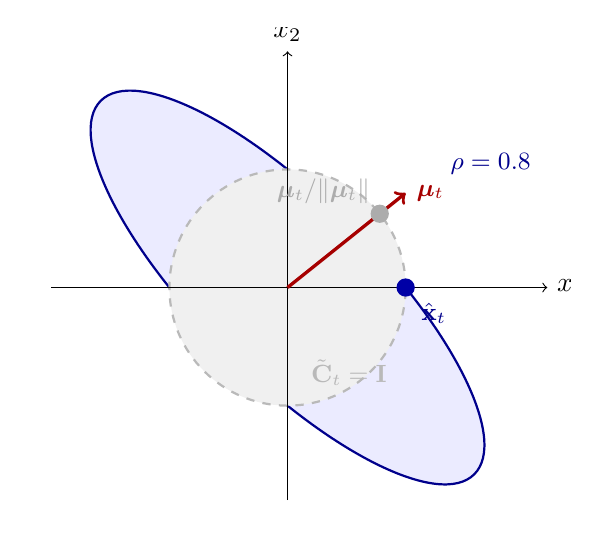
\begin{tikzpicture}[scale=1.5]
    \clip (-2.2, -2.0) rectangle (2.4, 2.2);

    % Blue ellipse: x^T C x = 1 with C = [[1, 0.8], [0.8, 1]], rho = 0.8.
    % Eigenvalues: lambda_+ = 1.8 along (1,1)/sqrt2 (compressed direction),
    %              lambda_- = 0.2 along (1,-1)/sqrt2 (stretched direction).
    % Semi-axes: 1/sqrt(1.8) ~ 0.7454 and 1/sqrt(0.2) ~ 2.2361.
    \begin{scope}[rotate=45]
      \fill[blue!8] (0,0) ellipse (0.7454 and 2.2361);
      \draw[blue!55!black, thick] (0,0) ellipse (0.7454 and 2.2361);
    \end{scope}

    % Grey circle: x^T I x = 1 (identity / proportional baseline).
    \fill[gray!12] (0,0) circle (1);
    \draw[dashed, gray!55, thick] (0,0) circle (1);

    % Axes.
    \draw[->] (-2.0, 0) -- (2.2, 0) node[right] {$x_1$};
    \draw[->] (0, -1.8) -- (0, 2.0) node[above] {$x_2$};

    % Signal vector mu = (1, 0.8).
    \draw[->, line width=1.2pt, red!65!black] (0,0) -- (1.0, 0.8)
      node[right, font=\small] {$\bm{\mu}_t$};

    % Proportional solution: mu/||mu|| ~ (0.7809, 0.6247).
    \fill[gray!65] (0.7809, 0.6247) circle (2.2pt);
    \node[gray!65, above left, font=\small] at (0.7809, 0.6247)
      {$\bm{\mu}_t/\|\bm{\mu}_t\|$};

    % Correlation-adjusted solution: hat_x = (1, 0).
    \fill[blue!65!black] (1.0, 0.0) circle (2.2pt);
    \node[blue!55!black, below right, font=\small] at (1.05, -0.05)
      {$\hat{\x}_t$};

    % Curve labels.
    \node[gray!55, font=\small\itshape] at (0.52, -0.72)
      {$\tilde{\C}_t = \I$};
    \node[blue!55!black, font=\small\itshape] at (1.72, 1.05)
      {$\rho = 0.8$};
  \end{tikzpicture}
  \caption{Geometric interpretation for $n = 2$ assets with signal
    $\bm{\mu}_t = (1,\,0.8)^\top$ (red arrow).
    \textbf{Grey circle}: feasible set under no correlation adjustment
    ($\tilde{\C}_t = \I$); the proportional solution $\bm{\mu}_t/\|\bm{\mu}_t\|$
    (grey dot) lies in the signal direction.
    \textbf{Blue ellipse}: feasible set $\{\x : \x^\top\tilde{\C}_t\x = 1\}$
    for $\rho = 0.8$; the correlation-adjusted solution
    $\hat{\x}_t = (1,\,0)^\top$ (blue dot) eliminates the position in
    asset~2, whose contribution to portfolio risk is already captured
    through the highly correlated asset~1.
    The ellipse is compressed in the correlated direction $(1,1)^\top$
    and stretched in the anti-correlated direction $(1,-1)^\top$.}
  \label{fig:ellipsoid}
\end{figure}

% ─────────────────────────────────────────────────────────────────────────────
\section{Factor Risk Models}
\label{sec:factor_models}
% ─────────────────────────────────────────────────────────────────────────────

The EWMA-plus-shrinkage framework described in Section~\ref{sec:approach}
estimates a full $n \times n$ correlation matrix at every timestamp and
regularises it toward the identity.  An alternative and complementary approach
is to posit a \emph{factor structure} for the covariance matrix: the returns
of $n$ assets are driven by a small number $k \ll n$ of common factors plus
independent idiosyncratic noise.  This section develops that structure, shows
how latent factors can be extracted from data via the Singular Value
Decomposition (SVD), derives an efficient solve via the
Sherman--Morrison--Woodbury identity, and describes a sliding-window estimator
parametrised by the pair $(n, k)$.

\subsection{The Factor Model Decomposition}
\label{sec:factor_model_decomp}

A factor risk model decomposes the $n \times n$ covariance matrix as
\begin{equation}
  \label{eq:factor_model}
  \bm{\Sigma} = \Bload\Ffac\Bload^\top + \Dspe,
\end{equation}
where
\begin{itemize}
  \item $\Bload \in \R^{n \times k}$ is the \emph{factor loading matrix}: column~$j$
    gives the sensitivity of each asset to factor~$j$;
  \item $\Ffac \in \R^{k \times k}$ is the \emph{factor covariance matrix}
    (positive definite), capturing how the $k$ factors co-vary with one
    another; and
  \item $\Dspe = \operatorname{diag}(d_1, \dots, d_n)$ with $d_i > 0$ is the
    \emph{idiosyncratic risk matrix}, capturing the asset-specific variance
    unexplained by the common factors.
\end{itemize}

The central assumption is $k \ll n$: the dominant systematic
sources of risk---market direction, sector exposures, style tilts, and so
on---are captured by a handful of factors, while the idiosyncratic component
$\Dspe$ is, by construction, uncorrelated across assets.  Because $k \ll n$,
the model reduces the number of free parameters from $O(n^2)$ to $O(nk)$,
making estimation far more tractable when the observation count $T$ is small
relative to $n$.

Classic \emph{explicit} factor models specify $\Bload$ and $\Ffac$ using
economic theory or commercial risk-factor vendors, such as the Fama--French
three-factor model \citep{fama1993}.  In the purely data-driven setting
explored here the factors are \emph{latent} and must be inferred from returns.

\begin{remark}
  When $\Ffac = \I_k$ and the columns of $\Bload$ are orthonormal,
  Eq.~\eqref{eq:factor_model} reduces to a principal-component
  decomposition of $\bm{\Sigma}$: each factor corresponds to a principal
  direction and its loading magnitude equals the corresponding eigenvalue.
\end{remark}

\subsection{Latent Factors via the Singular Value Decomposition}
\label{sec:svd_factors}

The most natural way to extract latent factors from a return matrix is the
Singular Value Decomposition \citep{golub1996}.  Let
$\mathbf{R} \in \R^{T \times n}$ be the matrix whose $(t, i)$ entry is the
volatility-adjusted return $\tilde{r}_{i,t}$.  Its thin SVD is
\begin{equation}
  \label{eq:svd}
  \mathbf{R} = \mathbf{U}\bm{\Sigma}_{\mathrm{sv}}\mathbf{V}^\top,
\end{equation}
where $\mathbf{U} \in \R^{T \times n}$ has orthonormal columns
($\mathbf{U}^\top\mathbf{U} = \I_n$),
$\bm{\Sigma}_{\mathrm{sv}} = \operatorname{diag}(\sigma_1, \dots, \sigma_n)$
with $\sigma_1 \geq \sigma_2 \geq \cdots \geq \sigma_n \geq 0$, and
$\mathbf{V} \in \R^{n \times n}$ is orthogonal.  The sample correlation matrix
(assuming unit-variance columns) satisfies
\begin{equation}
  \label{eq:svd_cov}
  \hat{\C} = \frac{1}{T}\mathbf{R}^\top\mathbf{R}
           = \frac{1}{T}\mathbf{V}\bm{\Sigma}_{\mathrm{sv}}^2\mathbf{V}^\top.
\end{equation}
The columns $\mathbf{v}_j$ of $\mathbf{V}$ are the \emph{latent factor
directions} in asset space: $\mathbf{v}_1$ points in the direction of maximum
variance, $\mathbf{v}_2$ in the direction of maximum residual variance
orthogonal to $\mathbf{v}_1$, and so on.  The scalar $\sigma_j^2 / T$ is the
variance explained by factor~$j$.

The Eckart--Young--Mirsky theorem \citep{eckart1936} guarantees that retaining
only the top-$k$ singular triplets gives the best rank-$k$ approximation to
$\mathbf{R}$ (and to $\hat{\C}$) in both the Frobenius and spectral norms:
\begin{equation}
  \label{eq:truncated_svd}
  \mathbf{R}_k = \mathbf{U}_k\bm{\Sigma}_k\mathbf{V}_k^\top,
  \qquad
  \hat{\C}^{(k)} = \frac{1}{T}\mathbf{V}_k\bm{\Sigma}_k^2\mathbf{V}_k^\top
                 + \hat{\Dspe},
\end{equation}
where $\mathbf{U}_k \in \R^{T \times k}$,
$\bm{\Sigma}_k = \operatorname{diag}(\sigma_1, \dots, \sigma_k)$,
$\mathbf{V}_k \in \R^{n \times k}$, and $\hat{\Dspe}$ is a diagonal correction
chosen so that $\hat{\C}^{(k)}$ has unit diagonal (i.e., is a valid
correlation matrix).

Identifying $\Bload = \mathbf{V}_k$ and
$\Ffac = \bm{\Sigma}_k^2/T$ establishes the correspondence with
Eq.~\eqref{eq:factor_model}: the latent factors are the right singular
vectors, the factor covariance is diagonal with entries $\sigma_j^2/T$, and
the idiosyncratic matrix $\hat{\Dspe}$ absorbs the residual variance.

\paragraph{Choosing $k$.}
A common heuristic is to retain enough components to explain a target fraction
$\theta$ of total variance:
\begin{equation}
  k^* = \min\!\left\{k : \frac{\sum_{j=1}^{k}\sigma_j^2}
                              {\sum_{j=1}^{n}\sigma_j^2} \geq \theta\right\}.
\end{equation}
Alternatively, the Marchenko--Pastur bulk edge \citep{marchenko1967} provides a
noise-floor threshold: retain only singular values exceeding
$\sigma_{\max}^{\mathrm{MP}} = \sigma_{\mathrm{noise}}\sqrt{(1 + \sqrt{n/T})^2}$,
where $\sigma_{\mathrm{noise}}$ is an estimate of the noise level.  Both
criteria typically select $k$ in the range $3$--$20$ for equity universes with
daily data.

\subsection{Efficient Inversion via the Sherman--Morrison--Woodbury Identity}
\label{sec:woodbury}

For large $n$, the direct solve $\hat{\C}^{(k)}\,\x = \muvec$ is expensive
because forming and factorising the full $n \times n$ matrix costs $O(n^3)$.
The factor structure permits a much cheaper path via the \emph{Woodbury matrix
identity} \citep{woodbury1950}:
\begin{equation}
  \label{eq:woodbury}
  \bigl(\Dspe + \Bload\Ffac\Bload^\top\bigr)^{-1}
  = \Dspe^{-1}
    - \Dspe^{-1}\Bload
      \underbrace{\bigl(\Ffac^{-1} + \Bload^\top\Dspe^{-1}\Bload\bigr)^{-1}}_{k \times k}
      \Bload^\top\Dspe^{-1}.
\end{equation}
Because $\Dspe$ is diagonal, $\Dspe^{-1}$ costs $O(n)$.  The bracketed
term is a $k \times k$ matrix whose inversion costs $O(k^3)$, and the
surrounding multiplications cost $O(kn)$.  The total cost is therefore
$O(k^3 + kn)$, which is $O(kn)$ for $k \ll n$---a dramatic improvement
over $O(n^3)$ when $n$ is large and $k$ is small.

\begin{remark}
  For the pure SVD factor model ($\Ffac = \bm{\Sigma}_k^2/T$,
  $\Bload = \mathbf{V}_k$), the Woodbury formula specialises to
  \begin{equation}
    \Bigl(\hat{\Dspe}
           + \tfrac{1}{T}\mathbf{V}_k\bm{\Sigma}_k^2\mathbf{V}_k^\top\Bigr)^{-1}
    = \hat{\Dspe}^{-1}
      - \hat{\Dspe}^{-1}\mathbf{V}_k
        \Bigl(T\bm{\Sigma}_k^{-2}
               + \mathbf{V}_k^\top\hat{\Dspe}^{-1}\mathbf{V}_k\Bigr)^{-1}
        \mathbf{V}_k^\top\hat{\Dspe}^{-1}.
  \end{equation}
  The inner matrix $T\bm{\Sigma}_k^{-2} + \mathbf{V}_k^\top\hat{\Dspe}^{-1}\mathbf{V}_k$
  is $k \times k$ and positive definite, admitting a stable Cholesky
  factorisation.
\end{remark}

The \emph{Sherman--Morrison formula} is the rank-$1$ special case ($k = 1$)
of the Woodbury identity:
\begin{equation}
  \label{eq:sherman_morrison}
  (\mathbf{A} + \mathbf{u}\mathbf{v}^\top)^{-1}
  = \mathbf{A}^{-1}
    - \frac{\mathbf{A}^{-1}\mathbf{u}\,\mathbf{v}^\top\mathbf{A}^{-1}}
           {1 + \mathbf{v}^\top\mathbf{A}^{-1}\mathbf{u}},
\end{equation}
valid whenever $1 + \mathbf{v}^\top\mathbf{A}^{-1}\mathbf{u} \neq 0$.  When
the factor model has $k = 1$ (a single dominant factor, e.g.\ the market), the
full matrix inverse follows from a single $n$-vector computation, making
the per-timestamp solve $O(n)$.

\subsection{A Sliding Window with $k$ Factors}
\label{sec:sliding_window}

The EWMA correlation estimator of Section~\ref{sec:corr} assigns
exponentially decaying weights to all past observations, maintaining a running
estimate that is updated at each timestamp---an \emph{infinite-memory}
estimator.  An alternative is the \emph{sliding window} (or rolling-window)
estimator, which restricts attention to a fixed block of the $W$ most recent
observations and assigns them equal weight.

\paragraph{Construction.}
At timestamp $t$, let $\mathbf{R}_t \in \R^{W \times n}$ denote the submatrix
of volatility-adjusted returns for the window $[t - W + 1,\, t]$ across all
$n$ assets.  Its truncated SVD retaining $k$ components is
\begin{equation}
  \label{eq:sliding_svd}
  \mathbf{R}_t \approx \mathbf{U}_{k,t}\bm{\Sigma}_{k,t}\mathbf{V}_{k,t}^\top,
\end{equation}
and the factor-based correlation estimate used for the solve at time $t$ is
\begin{equation}
  \label{eq:sliding_corr}
  \hat{\C}_t^{(W,k)}
  = \frac{1}{W}\mathbf{V}_{k,t}\bm{\Sigma}_{k,t}^2\mathbf{V}_{k,t}^\top
  + \hat{\Dspe}_t,
\end{equation}
with $\hat{\Dspe}_t$ chosen to enforce unit diagonal.  The system
$\hat{\C}_t^{(W,k)}\,\x_t = \muvec_t$ can then be solved efficiently using
the Woodbury identity from Section~\ref{sec:woodbury}.

\paragraph{Parameters and trade-offs.}
The pair $(W, k)$ jointly controls the estimator:
\begin{itemize}
  \item \textbf{Window length $W$.}  Longer windows yield more stable factor
    directions but adapt slowly to regime changes.  A common rule of thumb is
    $W \geq 2n$ to ensure the sample covariance is well-posed before
    truncation.
  \item \textbf{Number of factors $k$.}  Small $k$ (e.g.\ $1$--$5$) captures
    only the dominant systematic risk (market, sector), giving a smooth,
    low-variance estimate.  Larger $k$ (up to $\min(W, n)$) captures finer
    correlation structure at the cost of higher estimation noise.  The
    $k = 1$ case recovers the market-factor model; $k = n$ (full rank)
    recovers the standard sample correlation matrix.
\end{itemize}

\paragraph{Comparison with EWMA.}
The EWMA and sliding-window estimators exhibit complementary properties.
EWMA assigns exponentially decaying weights, which is well suited to tracking
smooth regime transitions; its estimate is never zero-weight and is always
influenced by distant past data to some degree.  The sliding window assigns
uniform weights within the window and zero outside it: this hard truncation
makes the estimator more responsive to sudden structural breaks but introduces
a discrete jump whenever a large observation enters or leaves the window.
Table~\ref{tab:ewma_vs_sliding} summarises the comparison.

\begin{table}[h]
  \centering
  \caption{EWMA correlation versus sliding-window factor model.}
  \label{tab:ewma_vs_sliding}
  \begin{tabular}{lll}
    \toprule
    \textbf{Property} & \textbf{EWMA (shrinkage)} & \textbf{Sliding window ($W$, $k$)} \\
    \midrule
    Observation weights & Exponential decay & Uniform within window \\
    Memory horizon      & Infinite (soft)   & Exactly $W$ steps (hard) \\
    Free parameters     & $\lambda$, $h_\rho$ & $W$, $k$ \\
    Covariance rank     & Full $n$          & At most $k$ (plus diagonal) \\
    Per-step solve cost & $O(n^3)$          & $O(k^3 + kn)$ \\
    Regime responsiveness & Gradual          & Sharp at boundary \\
    \bottomrule
  \end{tabular}
\end{table}

% ─────────────────────────────────────────────────────────────────────────────
\section{Available Analytics}
\label{sec:analytics}
% ─────────────────────────────────────────────────────────────────────────────

The library exposes two layers of analytics: optimizer-level diagnostics that
introspect the numerical behaviour of the solve at each timestamp, and
portfolio-level analytics that measure the risk-adjusted performance of the
resulting positions.

\subsection{Optimizer-Level Diagnostics}
\label{sec:diagnostics}

The following properties are available on a \texttt{BasanosEngine} instance.
Each returns a Polars \texttt{DataFrame} indexed by timestamp.

\subsubsection{Condition Number}

The condition number $\kappa(\tilde{\C}_t)$ of the shrunk correlation matrix
quantifies numerical sensitivity of the solve:
\begin{equation}
  \kappa(\tilde{\C}_t) = \frac{\lambda_{\max}(\tilde{\C}_t)}
                              {\lambda_{\min}(\tilde{\C}_t)},
\end{equation}
where $\lambda_{\max}$ and $\lambda_{\min}$ are the largest and smallest
eigenvalues respectively.  A value near $n$ is expected for a healthy,
lightly shrunk matrix.  Values above $10^{12}$ trigger a warning and indicate
that positions may be numerically unreliable.

\subsubsection{Effective Rank}

The effective rank measures the true dimensionality of the portfolio by
computing the Shannon entropy of the eigenvalue spectrum of $\tilde{\C}_t$:
\begin{equation}
  \eff(\tilde{\C}_t) = \exp\!\left(-\sum_{i=1}^{n} p_i \ln p_i\right),
  \quad p_i = \frac{\lambda_i}{\sum_j \lambda_j},
\end{equation}
where $\lambda_i$ are the eigenvalues of $\tilde{\C}_t$.  A value of $n$
indicates a perfectly uniform spectrum (identity-like matrix, assets
effectively independent).  A value near 1 indicates a rank-1 matrix dominated
by a single common factor.  Monitoring effective rank over time reveals whether
the portfolio's correlation structure is diversified or concentrated.

\subsubsection{Solver Residual}

After solving the system in Eq.~\eqref{eq:system}, the Euclidean residual
\begin{equation}
  \varepsilon_t = \norm{\tilde{\C}_t\,\x_t - \muvec_t}_2
\end{equation}
measures numerical accuracy.  For a well-posed, well-conditioned system,
$\varepsilon_t$ should be near machine epsilon ($\approx 10^{-15}$).  Large
residuals flag near-singular matrices or solver fallback from Cholesky to LU.

\subsubsection{Signal Utilisation}

For each asset $i$, signal utilisation measures the fraction of the original
signal that survives the correlation filter:
\begin{equation}
  u_{i,t} = \frac{(\tilde{\C}_t^{-1}\muvec_t)_i}{\mu_{i,t}}.
\end{equation}
When $\tilde{\C}_t = \I_n$, all assets have $u_{i,t} = 1$.  Off-diagonal
correlations attenuate some assets ($u_{i,t} < 1$) and may amplify
negatively correlated ones ($u_{i,t} > 1$).  This diagnostic reveals
which assets are most affected by the correlation adjustment and by how much.

\subsubsection{Position Leverage}

Gross leverage at each timestamp is the L1 norm of the cash-position vector:
\begin{equation}
  L_t = \norm{\mathbf{p}_t}_1 = \sum_{i=1}^{n} \abs{p_{i,t}}.
\end{equation}
Monitoring leverage over time reveals whether the correlation adjustment
amplifies or dampens total exposure relative to the signal-proportional
baseline.

\subsubsection{Risk Position}

The risk position is the unscaled cash position before dividing by
per-asset volatility:
\begin{equation}
  x_{i,t}^\text{risk} = p_{i,t} \times \sigma_{i,t}.
\end{equation}
It is returned as a \texttt{DataFrame} with the same shape as
\texttt{cash\_position}, and is useful for cross-asset comparison on a
common volatility-adjusted scale.

\subsection{Signal Quality Metrics}
\label{sec:signal_quality}

The following properties are available on a \texttt{BasanosEngine} instance
and evaluate the signal's cross-sectional predictive content independently
of any portfolio construction.  Each IC observation is computed as a
cross-sectional statistic over the active assets at each timestamp.

\subsubsection{Information Coefficient (IC)}

The IC at timestamp $t$ is the Pearson correlation between the signal
$\muvec_t$ and the one-step-ahead asset returns $\mathbf{r}_{t+1}$:
\begin{equation}
  \mathrm{IC}_t = \operatorname{corr}(\muvec_t,\, \mathbf{r}_{t+1}).
\end{equation}
The property \texttt{engine.ic} returns a Polars \texttt{DataFrame} of
per-timestamp IC values.

\subsubsection{Rank IC}

The Rank IC is the Spearman rank correlation between $\muvec_t$ and
$\mathbf{r}_{t+1}$.  It is more robust to outliers than the Pearson IC and
is the standard metric for evaluating signal quality in the quantitative
finance literature.  Available as \texttt{engine.rank\_ic}.

\subsubsection{Summary Statistics}

\begin{itemize}
  \item \texttt{engine.icir} --- Information Coefficient Information Ratio:
    $\mathrm{ICIR} = \bar{\mathrm{IC}} / \hat{\sigma}_\mathrm{IC}$, where
    $\bar{\mathrm{IC}}$ is the mean and $\hat{\sigma}_\mathrm{IC}$ the
    standard deviation of the IC time series.
  \item \texttt{engine.rank\_ic\_mean} --- Mean of the Rank IC series.
  \item \texttt{engine.rank\_ic\_std} --- Standard deviation of the Rank IC
    series.
\end{itemize}

\subsection{Portfolio-Level Analytics}
\label{sec:portfolio_analytics}

After positions are computed, a \texttt{Portfolio} object provides a
comprehensive set of performance analytics.  The key properties are
summarised below.

\subsubsection{P\&L and NAV}

\begin{itemize}
  \item \textbf{profits} --- Per-asset daily cash P\&L:
    $\pi_{i,t} = p_{i,t-1}\,(S_{i,t}/S_{i,t-1} - 1)$.
  \item \textbf{profit} --- Aggregate portfolio daily P\&L:
    $\Pi_t = \sum_i \pi_{i,t}$.
  \item \textbf{nav\_accumulated} --- Cumulative additive NAV:
    $\text{NAV}_t = \text{AUM} + \sum_{s\leq t}\Pi_s$.
  \item \textbf{nav\_compounded} --- Compounded NAV:
    $\text{NAV}_t^c = \text{AUM}\,\prod_{s\leq t}(1 + \Pi_s/\text{AUM})$.
\end{itemize}

\subsubsection{Risk and Drawdown}

\begin{itemize}
  \item \textbf{highwater} --- Running maximum of the accumulated NAV.
  \item \textbf{drawdown} --- Distance from the high-water mark:
    $\text{DD}_t = (\text{HWM}_t - \text{NAV}_t)/\text{HWM}_t$.
  \item \textbf{returns} --- Daily return series: $r_t = \Pi_t / \text{AUM}$.
\end{itemize}

\subsubsection{Performance Attribution}

Following \citet{brinson1986}, Basanos decomposes the portfolio return into
two orthogonal components:
\begin{description}
  \item[Tilt (allocation effect)] The return due to time-averaged static
    weights $\bar{\mathbf{p}} = T^{-1}\sum_t \mathbf{p}_t$.  This measures
    the passive, structural exposure of the portfolio.
  \item[Timing (selection effect)] The return due to dynamic deviations from
    the static tilt: $\Delta\mathbf{p}_t = \mathbf{p}_t - \bar{\mathbf{p}}$.
    This isolates the pure signal-driven, time-varying component of performance.
\end{description}
Together they provide a clean decomposition:
\begin{equation}
  \Pi_t = \Pi_t^\text{tilt} + \Pi_t^\text{timing}.
\end{equation}
A signal with no edge will show a flat or negative timing NAV even if the
tilt NAV is positive (due to incidental factor exposures), which directly
answers the question of whether the dynamic component adds value.

\subsubsection{Turnover}

One-way portfolio turnover at time $t$ is
\begin{equation}
  \tau_t = \frac{1}{2}\,\norm{\mathbf{p}_t - \mathbf{p}_{t-1}}_1.
\end{equation}
High turnover relative to signal magnitude is a warning sign: either the
signal is noisy or the correlation matrix is changing rapidly.  Turnover also
provides an upper bound on the transaction costs that would arise in
production.

\subsection{Statistical Metrics}
\label{sec:stats}

The \texttt{Stats} class (available as \texttt{portfolio.stats}) computes
the following metrics on the portfolio returns series.  All metrics are
available both for the aggregate portfolio and on a per-asset basis.

\paragraph{Risk-adjusted performance.}
\begin{itemize}
  \item \textbf{Sharpe ratio} \citep{sharpe1966}:
    $S = \sqrt{252}\,\bar{r}/\hat{\sigma}$, where $\bar{r}$ is the mean
    daily return and $\hat{\sigma}$ is the sample standard deviation.
  \item \textbf{Calmar ratio}: annualised return divided by maximum drawdown.
  \item \textbf{Recovery factor}: total return divided by maximum drawdown.
\end{itemize}

\paragraph{Risk metrics.}
\begin{itemize}
  \item \textbf{Volatility}: annualised standard deviation of daily returns.
  \item \textbf{Value at Risk (VaR)}: parametric VaR at a given confidence
    level, computed from the sample mean and standard deviation assuming
    Gaussian returns.
  \item \textbf{Conditional Value at Risk (CVaR)} \citep{rockafellar2000}:
    expected shortfall beyond the VaR threshold.
  \item \textbf{Maximum drawdown} and \textbf{average drawdown}: measures
    of peak-to-trough loss.
  \item \textbf{Maximum drawdown duration}: longest period spent below the
    high-water mark.
\end{itemize}

\paragraph{Distributional properties.}
\begin{itemize}
  \item Mean, skewness, excess kurtosis.
  \item Best and worst single-day returns.
\end{itemize}

\paragraph{Win/loss analysis.}
\begin{itemize}
  \item Win rate: fraction of days with positive P\&L.
  \item Monthly win rate: fraction of calendar months with positive P\&L.
  \item Profit factor: gross profit divided by gross loss.
  \item Payoff ratio: average win divided by average loss.
  \item Average win and average loss.
\end{itemize}

\paragraph{Relative performance.}
\begin{itemize}
  \item Up-capture and down-capture ratios versus a user-supplied benchmark.
  \item Worst $k$-period windows for stress testing.
\end{itemize}

\paragraph{Rolling metrics.}
\begin{itemize}
  \item Rolling Sharpe ratio and rolling volatility time series, both with
    configurable window sizes.  These reveal whether performance is
    concentrated in a short regime or consistently earned across the history.
\end{itemize}

\subsection{Visualisations and Reports}
\label{sec:viz}

The \texttt{Plots} class (available as \texttt{portfolio.plots}) produces
interactive Plotly figures:

\begin{itemize}
  \item \textbf{NAV snapshot} (\texttt{snapshot()}): cumulative NAV and
    drawdown dashboard.
  \item \textbf{Lead/lag IR plot} (\texttt{lead\_lag\_ir\_plot(start, end)}):
    Sharpe ratio as a function of position lag, revealing whether the signal
    has predictive power ahead of or behind the positions as submitted.  A
    peak at lag~0 is the expected result for a correctly timed signal.
  \item \textbf{Lagged performance} (\texttt{lagged\_performance\_plot(...)}):
    NAV curves for multiple position lags overlaid for comparison.
  \item \textbf{Rolling Sharpe} (\texttt{rolling\_sharpe\_plot(window)}): time
    series of rolling Sharpe ratio to assess performance stability.
  \item \textbf{Rolling volatility} (\texttt{rolling\_volatility\_plot(...)}):
    time series of rolling annualised volatility.
  \item \textbf{Annual Sharpe} (\texttt{annual\_sharpe\_plot()}): bar chart of
    Sharpe ratio by calendar year, useful for detecting single-year anomalies.
  \item \textbf{Correlation heatmap} (\texttt{correlation\_heatmap()}):
    time-averaged asset correlation matrix.
\end{itemize}

A one-call \texttt{Report} object (\texttt{portfolio.report}) renders all of
the above as a self-contained, dark-themed HTML document that can be served
via an API or saved to disk.

% ─────────────────────────────────────────────────────────────────────────────
\section{Usage Example}
\label{sec:usage}
% ─────────────────────────────────────────────────────────────────────────────

\subsection{Development Infrastructure}

Basanos is developed using the \textbf{Rhiza} framework---a curated collection
of reusable project-template files, Makefile targets, and CI/CD workflows
designed to standardise modern Python library development.  Rhiza manages
dependency resolution via \texttt{uv}, enforces code style with \texttt{ruff},
runs the test suite under \texttt{pytest} with coverage, and automates
packaging and release workflows.  A downstream project stays synchronised with
the upstream Rhiza template through a periodic sync step that propagates
improvements to the shared tooling without touching library-specific logic.
This separation between domain code and build infrastructure keeps the
repository focused on the mathematical and analytical core while benefiting
from continuously maintained development tooling.

\subsection{End-to-End Example}

The following example illustrates the complete workflow from price data and a
signal to a performance report.

\begin{lstlisting}[language=Python,
                   caption={End-to-end example: optimization and analytics.}]
import numpy as np
import polars as pl
from basanos.math import BasanosConfig, BasanosEngine

# --- Synthetic data ---
n_days = 500
rng = np.random.default_rng(42)
dates = pl.date_range(
    pl.date(2022, 1, 1),
    pl.date(2022, 1, 1) + pl.duration(days=n_days - 1),
    eager=True,
)
prices = pl.DataFrame({
    "date":  dates,
    "AAPL":  100.0 + np.cumsum(rng.normal(0, 1.0, n_days)),
    "GOOGL": 150.0 + np.cumsum(rng.normal(0, 1.2, n_days)),
    "MSFT":  200.0 + np.cumsum(rng.normal(0, 0.9, n_days)),
})
mu = pl.DataFrame({
    "date":  dates,
    "AAPL":  np.tanh(rng.normal(0, 0.5, n_days)),
    "GOOGL": np.tanh(rng.normal(0, 0.5, n_days)),
    "MSFT":  np.tanh(rng.normal(0, 0.5, n_days)),
})

# --- Configuration ---
cfg = BasanosConfig(
    vola=16,    # EWMA half-life for volatility (days)
    corr=64,    # EWMA half-life for correlations (>= vola)
    clip=3.5,   # Clipping threshold (standard deviations)
    shrink=0.6, # Shrinkage retention weight lambda
    aum=1e6,    # Assets under management
)

# --- Optimization ---
engine    = BasanosEngine(prices=prices, mu=mu, cfg=cfg)
positions = engine.cash_position       # Optimized cash positions
status    = engine.position_status     # Per-row reason code (warmup/zero_signal/degenerate/valid)

# --- Optimizer diagnostics ---
kappa    = engine.condition_number     # Matrix condition over time
eff_rank = engine.effective_rank       # Effective rank over time
residual = engine.solver_residual      # Solve residual over time
utilisation = engine.signal_utilisation  # Per-asset signal utilisation

# --- Signal quality metrics ---
ic_series = engine.ic                  # Per-timestamp Pearson IC
rank_ic   = engine.rank_ic            # Per-timestamp Rank IC
print(engine.icir)                    # IC Information Ratio
print(engine.naive_sharpe)            # Sharpe under proportional sizing

# --- Portfolio analytics ---
portfolio = engine.portfolio
print(portfolio.stats.sharpe()["returns"])        # Annualised Sharpe ratio
print(portfolio.stats.max_drawdown()["returns"])  # Maximum drawdown
decomp = portfolio.tilt_timing_decomp  # Tilt vs. timing NAV curves

# --- Visualisation ---
fig = portfolio.plots.snapshot()           # NAV + drawdown
fig = portfolio.plots.lead_lag_ir_plot(-5, 15)  # Lead/lag Sharpe
portfolio.report.save("output/report")    # Full HTML report
\end{lstlisting}

% ─────────────────────────────────────────────────────────────────────────────
\section{Shrinkage as a Sensitivity Analysis}
\label{sec:sensitivity}
% ─────────────────────────────────────────────────────────────────────────────

Because $\lambda = 0$ recovers signal-proportional sizing and $\lambda = 1$
uses the raw EWMA matrix, sweeping $\lambda$ between these extremes provides
a direct measurement of how much value correlation adjustment adds.
Basanos exposes this as the method
\texttt{engine.sharpe\_at\_shrink($\lambda$)}, which re-runs the optimiser
with a given $\lambda$ and returns the annualised Sharpe ratio.

A complementary baseline is \texttt{engine.naive\_sharpe}, which computes the
Sharpe ratio when each asset is positioned proportionally to its signal
with no correlation adjustment (equivalent to $\lambda = 0$).  Together,
\texttt{naive\_sharpe}, \texttt{sharpe\_at\_shrink(0.0)}, and
\texttt{sharpe\_at\_shrink(cfg.shrink)} form a three-point diagnostic that
separates raw signal skill from the value added by correlation routing.

A typical sweep over $\lambda \in [0, 1]$ with fixed prices and signals
yields a Sharpe curve that either:
\begin{enumerate}
  \item \textbf{Peaks at an interior $\lambda$}: correlation adjustment
    adds value, and the optimal intensity is data-driven.
  \item \textbf{Monotonically decreases from $\lambda = 0$}: the signal is
    already well-diversified and the EWMA correlation estimate introduces
    estimation noise.
  \item \textbf{Monotonically increases toward $\lambda = 1$}: a strong
    correlation structure exists in the data that the signal does not yet
    exploit.
\end{enumerate}
This diagnostic is a fast, parameter-free sanity check before committing
to a production deployment.

% ─────────────────────────────────────────────────────────────────────────────
\section{Computational Characteristics}
\label{sec:compute}
% ─────────────────────────────────────────────────────────────────────────────

Let $N$ denote the number of assets and $T$ the number of timestamps.

\begin{table}[h]
  \centering
  \caption{Computational complexity of the main pipeline steps.}
  \label{tab:complexity}
  \begin{tabular}{lll}
    \toprule
    \textbf{Step} & \textbf{Complexity} & \textbf{Notes} \\
    \midrule
    Volatility adjustment  & $O(TN)$   & EWMA per asset, linear in both \\
    Correlation estimation & $O(TN^2)$ & $N^2$ pairs; parallelised via \texttt{lfilter} \\
    Linear solve (per row) & $O(N^3)$  & Cholesky; total $O(TN^3)$ \\
    Portfolio analytics    & $O(TN)$   & Element-wise P\&L and NAV \\
    \bottomrule
  \end{tabular}
\end{table}

Memory usage is dominated by storing all correlation matrices:
$O(TN^2)$ \texttt{float64} values, approximately
$8 T N^2$ bytes.  For $N=50$, $T=1260$ (five years of daily data), this
is approximately 25~MB.

Practical limits on an 8~GB workstation:
\begin{itemize}
  \item $N \leq 150$, $T \leq 1260$: seconds.
  \item $N \leq 250$, $T \leq 2520$: 10--60~seconds, \textasciitilde12~GB RAM.
  \item $N > 500$: exceeds 16~GB RAM.
\end{itemize}

% ─────────────────────────────────────────────────────────────────────────────
\section{Conclusion}
\label{sec:conclusion}
% ─────────────────────────────────────────────────────────────────────────────

This paper has presented the signal assessment problem that motivates the
Basanos library, the correlation-aware linear-solve approach it uses to
handle non-trivial portfolio geometry, and the suite of analytics it makes
available at both the optimizer and portfolio level.

The key insight is that raw signal-proportional sizing conflates two
distinct quantities: (i) the predictive content of the signal and (ii) its
interaction with the portfolio correlation structure.  By inverting the
correlation matrix explicitly---through a normalised solution of
$\tilde{\C}_t\,\x_t = \muvec_t$---Basanos disentangles these effects.
The result is a clean measurement surface on which signal quality can be
assessed through standard metrics: Sharpe ratio, drawdown, tilt/timing
decomposition, and lead/lag analysis.

The deliberate absence of hard constraints is a feature, not a
limitation.  It means the realised P\&L measures the signal's intrinsic
edge rather than its interaction with a production constraint set.  A signal
that cannot pass this first hurdle is unlikely to survive the additional
friction of a full production system.

\appendix

% ─────────────────────────────────────────────────────────────────────────────
\section{Configuration Parameters}
\label{app:config}
% ─────────────────────────────────────────────────────────────────────────────

\begin{table}[h]
  \centering
  \caption{\texttt{BasanosConfig} parameters and their roles.}
  \label{tab:config}
  \begin{tabular}{>{\ttfamily}lp{6cm}l}
    \toprule
    \normalfont\textbf{Parameter} & \textbf{Description} & \textbf{Default} \\
    \midrule
    vola   & EWMA half-life for volatility (days). Required. & --- \\
    corr   & EWMA half-life for correlation (days, $\geq$ vola). Required. & --- \\
    clip   & Clipping threshold for vol-adjusted returns ($> 0$). Required. & --- \\
    shrink & Shrinkage retention weight $\lambda \in [0,1]$. Required. & --- \\
    aum    & Assets under management for position scaling ($> 0$). Required. & --- \\
    denom\_tol & Zero threshold for normalisation denominator. & $10^{-12}$ \\
    position\_scale & Multiplicative scaling applied to risk positions. & $10^6$ \\
    min\_corr\_denom & Guard threshold for EWMA correlation denominator. & $10^{-14}$ \\
    max\_nan\_fraction & Maximum tolerated null fraction per asset column. & $0.9$ \\
    cost\_per\_unit & One-way trading cost per unit of position change. & $0.0$ \\
    max\_turnover & Optional L1 turnover budget per period (cash units). & \texttt{None} \\
    covariance\_config & Covariance mode: \texttt{EwmaShrinkConfig} or \texttt{SlidingWindowConfig}. & \texttt{EwmaShrinkConfig()} \\
    \bottomrule
  \end{tabular}
\end{table}

% ─────────────────────────────────────────────────────────────────────────────
\section{Optimizer Diagnostics Summary}
\label{app:diagnostics}
% ─────────────────────────────────────────────────────────────────────────────

\begin{table}[h]
  \centering
  \caption{Properties available on \texttt{BasanosEngine}.}
  \label{tab:diagnostics}
  \begin{tabular}{>{\ttfamily}lp{7.5cm}}
    \toprule
    \normalfont\textbf{Property} & \textbf{Description} \\
    \midrule
    cash\_position    & Optimized cash positions; the primary output. \\
    position\_status  & Per-row reason code: \texttt{warmup}, \texttt{zero\_signal}, \texttt{degenerate}, or \texttt{valid}. \\
    risk\_position    & Cash positions multiplied by per-asset volatility; positions on a common vol-adjusted scale. \\
    position\_leverage & L1 norm of cash positions (gross leverage) per timestamp. \\
    condition\_number & Condition number $\kappa(\tilde{\C}_t)$ per timestamp. \\
    effective\_rank   & Entropy-based effective rank of $\tilde{\C}_t$ per timestamp. \\
    solver\_residual  & Euclidean residual $\|\tilde{\C}_t\x_t - \muvec_t\|_2$ per timestamp. \\
    signal\_utilisation & Per-asset fraction of signal surviving the correlation filter. \\
    portfolio         & \texttt{Portfolio} instance built from the optimized positions. \\
    cor               & Dict of per-timestamp raw EWMA correlation matrices. \\
    cor\_tensor       & All correlation matrices as an $(T, N, N)$ NumPy array. \\
    vola              & Per-asset EWMA volatility estimates. \\
    ret\_adj          & Volatility-adjusted, clipped log returns. \\
    ic                & Per-timestamp Pearson IC (signal vs.\ forward returns). \\
    rank\_ic          & Per-timestamp Spearman Rank IC. \\
    icir              & Scalar IC Information Ratio: mean IC / std IC. \\
    rank\_ic\_mean    & Mean of the Rank IC time series. \\
    rank\_ic\_std     & Standard deviation of the Rank IC time series. \\
    naive\_sharpe     & Sharpe ratio under signal-proportional sizing (no correlation adjustment). \\
    \bottomrule
  \end{tabular}
\end{table}

% ─────────────────────────────────────────────────────────────────────────────
\bibliographystyle{plainnat}
\bibliography{basanos}
% ─────────────────────────────────────────────────────────────────────────────

\end{document}
